%% 062Analyse.tex
%% $Id: 062Analyse.tex 4 2005-10-10 20:51:21Z bless $
%%

%% ==============================
\subsection{Angaben der Probanden}
%% ==============================

\begin{figure}[htbp] 
	\centering
	\begin{minipage}[t]{0.8\textwidth}
		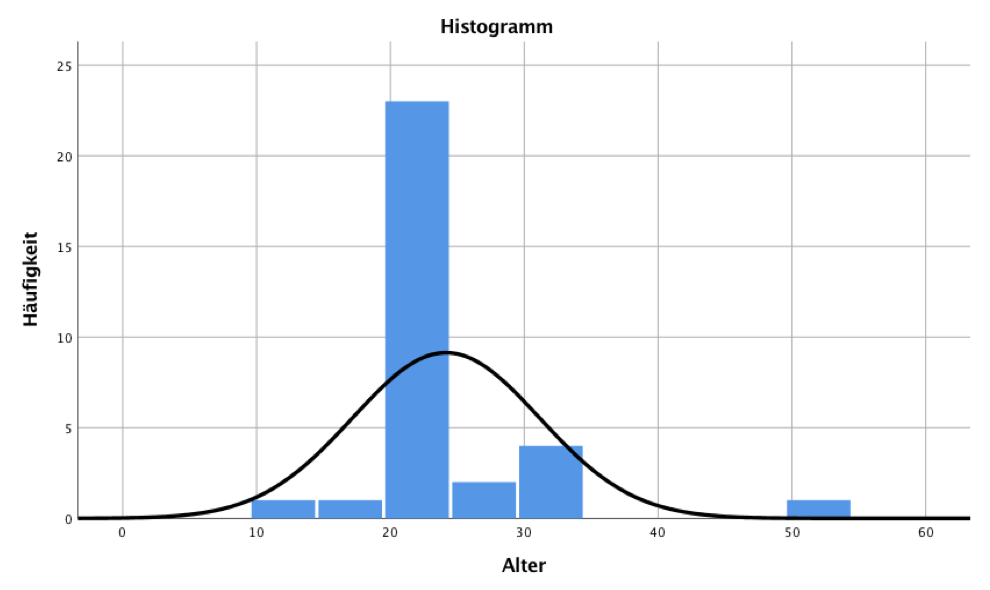
\includegraphics[width=\textwidth]{pics/analyse/person/alter.png}
	\end{minipage}
	\begin{minipage}[t]{0.8\textwidth}
		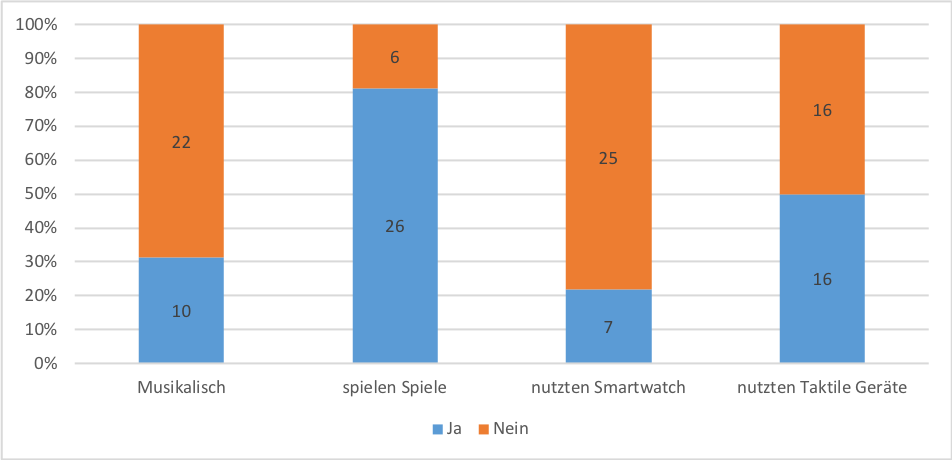
\includegraphics[width=\textwidth]{pics/analyse/person/questions.png}
	\end{minipage}
	\caption{Alter aller Probanden (links) und Auswertung der Fragen (rechts)}
	\label{fig:AngabenZurPerson}
\end{figure}

Nach der Befragung der Probanden hat sich ergeben \autoref{fig:AngabenZurPerson}, dass 31\% musikalisch sind, 81\% gelegentlich Computerspiele spielen. 21\% haben schon mal eine Smartwatch benutzt und genau die h{\"a}lfte haben schon mal taktile Ger{\"a}te benutzt.

%% ==============================
\subsection{Initialisierung der Grenzen}
%% ==============================
\label{ch:Evolution{\"a}rer Algorithmus:sec:Studiendesign}

\begin{figure}[htbp] 
            \centering
   	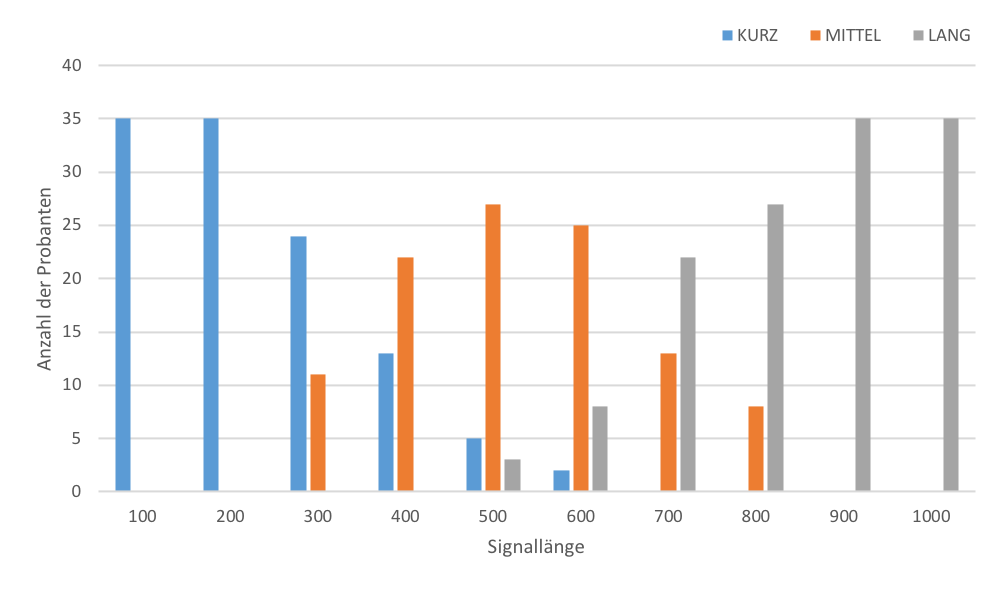
\includegraphics[width=0.8\textwidth]{pics/analyse/Initialisierung.png}
	\caption{TODO}
	\label{fig:Initialisierung}
\end{figure}

F{\"u}r die Bestimmung der Grenzen von Kurz, Mittel und Lang hat der Benutzer 10 Signale zu der jeweiligen Kategorie einordnen sollen. 
Da man bei 16\% der Probanden bei diesem Schritt keine eindeutigen Grenzen bestimmen konnte, musste der Schritt ein weiteres mal wiederholt werden. Die Auswertung der {\"u}bertragung hat ergeben, dass es im Durschnitt 300ms gedauert hat, bis das Signal {\"u}bertragen worden ist.

Obwohl die 10 normalverteilten Signale in zuf{\"a}lliger Reihenfolge abgespielt wurden, wurde bei 84\% aller Probanden die zehn Signale so bewertet, dass zuerst alle Kurz, gefolgt von nur Mittel und anschlie{\ss}end nur Lang bewertet wurden. 
Die restlichen Probanden haben an den Grenzen der Signaltypen nur \textit{Kurz} und \textit{Mittel} oder \textit{Mittel} und \textit{Lang} vertauscht.
%von Kurz und Mittel oder Mittel und Lang vertauscht gehabt.

%Au{\ss}erdem ist bei 84\% aller Probanden die Zuordnung der Kategorie zu den Signalen so bewertet worden, dass zuerst eine Anzahl von Signalen als Kurz, gefolgt von einer weiteren Anzahl als Mittel und schlie{\ss}lich der Rest als Lang erkannt worden ist.
%dass zuerst alle Signale als Kurz, gefolgt von nur Signale als Mittel und schlie{\ss}lich nur Signale vom Langen . 

%Die restlichen 16\% der Probanden haben an den Grenzen der Signaltypen nur ein Signal vom Kurz und Mittel oder Mittel und Lang vertauscht gehabt.

In der Auswertung \autoref{fig:Initialisierung} haben sich drei Normalverteilungen gebildet. 
Daraus kann man entnehmen, dass Werte 100ms und  200 ms eindeutig als Kurz, sowie auch Werte 900ms und 1000ms als Lang erkannt worden sind. 
Einen eindeutigen Hochpunkt f{\"u}r Mittel hat man bei dem Wert von 500ms, dennoch gab es einige Probanden f{\"u}r die dieser Wert noch als Kurz oder Lang empfunden wurde. 

Aus dem Diagramm kann man sehr sch{\"o}n erkennen, dass man eine Personalisierung von Vibrationen ben{\"o}tigen k{\"o}nnte, da man au{\ss}er den R{\"a}ndern keine eindeutige Zuweisung von \textit{Kurz}, \textit{Mittel} oder \textit{Lang} unter allen Probanden bestimmen konnte. 
Man kann zwar im Vorfeld Werte f{\"u}r Signale definieren, wie es derzeitig einige Firmen machen, diese Werte k{\"o}nnten jedoch von Personen unterschiedlich wahrgenommen werden.
%Aus dem Diagramm kann man sehr sch{\"o}n erkennen, dass man Werte zwar im Vorfeld selbst definieren kann, diese Werte k{\"o}nnten unter verschiedenen Probanden jedoch anders wahrgenommen werden und es wei{\ss}t darauf hin, dass man sehr wohl eine Personalisierung von Vibrationen ben{\"o}tigen k{\"o}nnte. 

%% ==============================
\subsection{Auswertung der Iterationen des Algorithmus}
%% ==============================


\paragraph{Verlauf der Grenzen}

\begin{figure}[htbp] 
	\centering
	\begin{minipage}[t]{0.8\textwidth}
		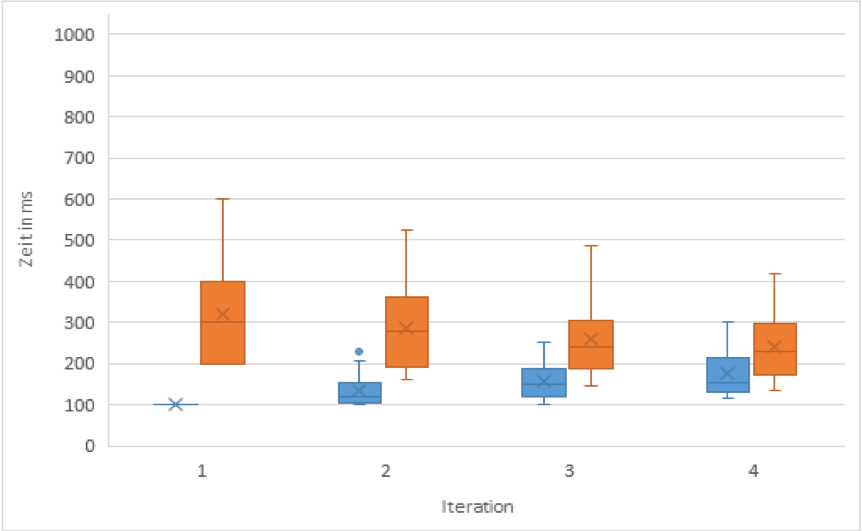
\includegraphics[width=\textwidth]{pics/analyse/algo/MinMax/sonstige/KurzMinMax2.png}
	\end{minipage}
	\begin{minipage}[t]{0.8\textwidth}
		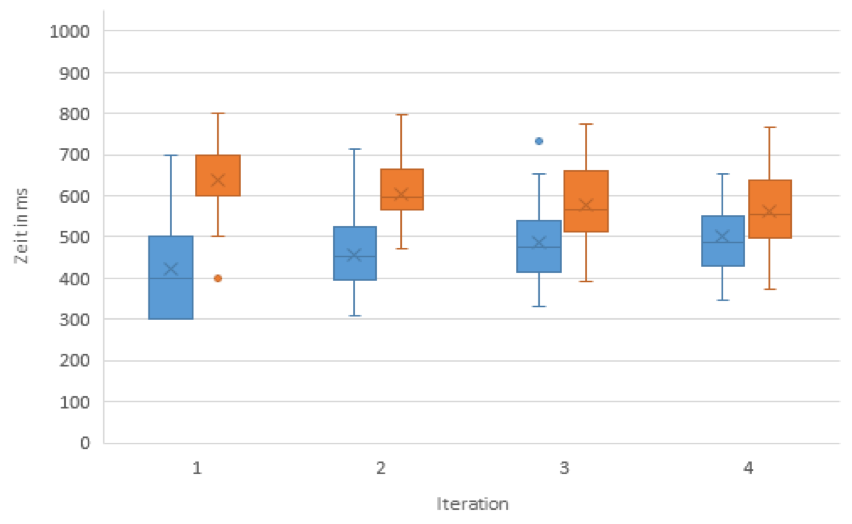
\includegraphics[width=\textwidth]{pics/analyse/algo/MinMax/sonstige/MittelMinMax2.png}
	\end{minipage}
\begin{minipage}[t]{0.8\textwidth}
		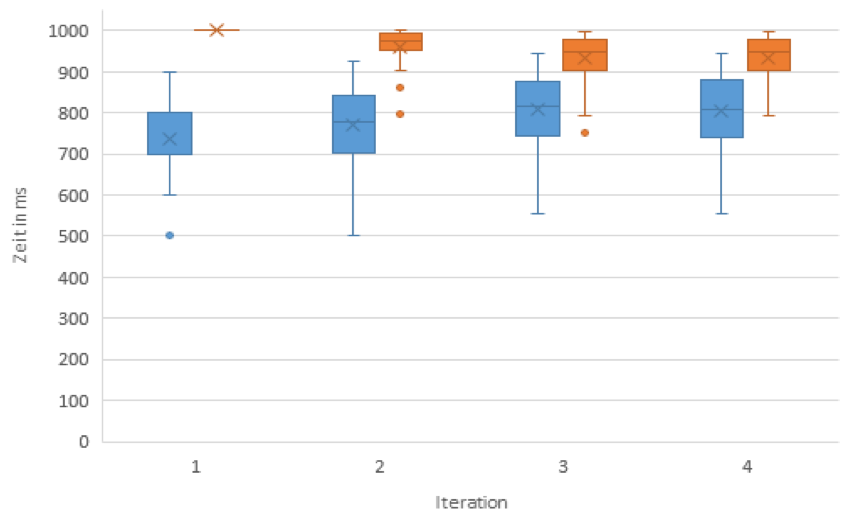
\includegraphics[width=\textwidth]{pics/analyse/algo/MinMax/sonstige/LangMinMax2.png}
	\end{minipage}
	\caption{Darstellung des Minimum (in blau) und Maximum (in rot) im Verlauf der 4 Iterationen des Algorithmus. Das erste Bild zeit Kurz, gefolgt von Mittel und Lang.}
	\label{fig:MinMaxSignale}
\end{figure}

%\begin{figure}[htbp] 
%	   \centering
%   	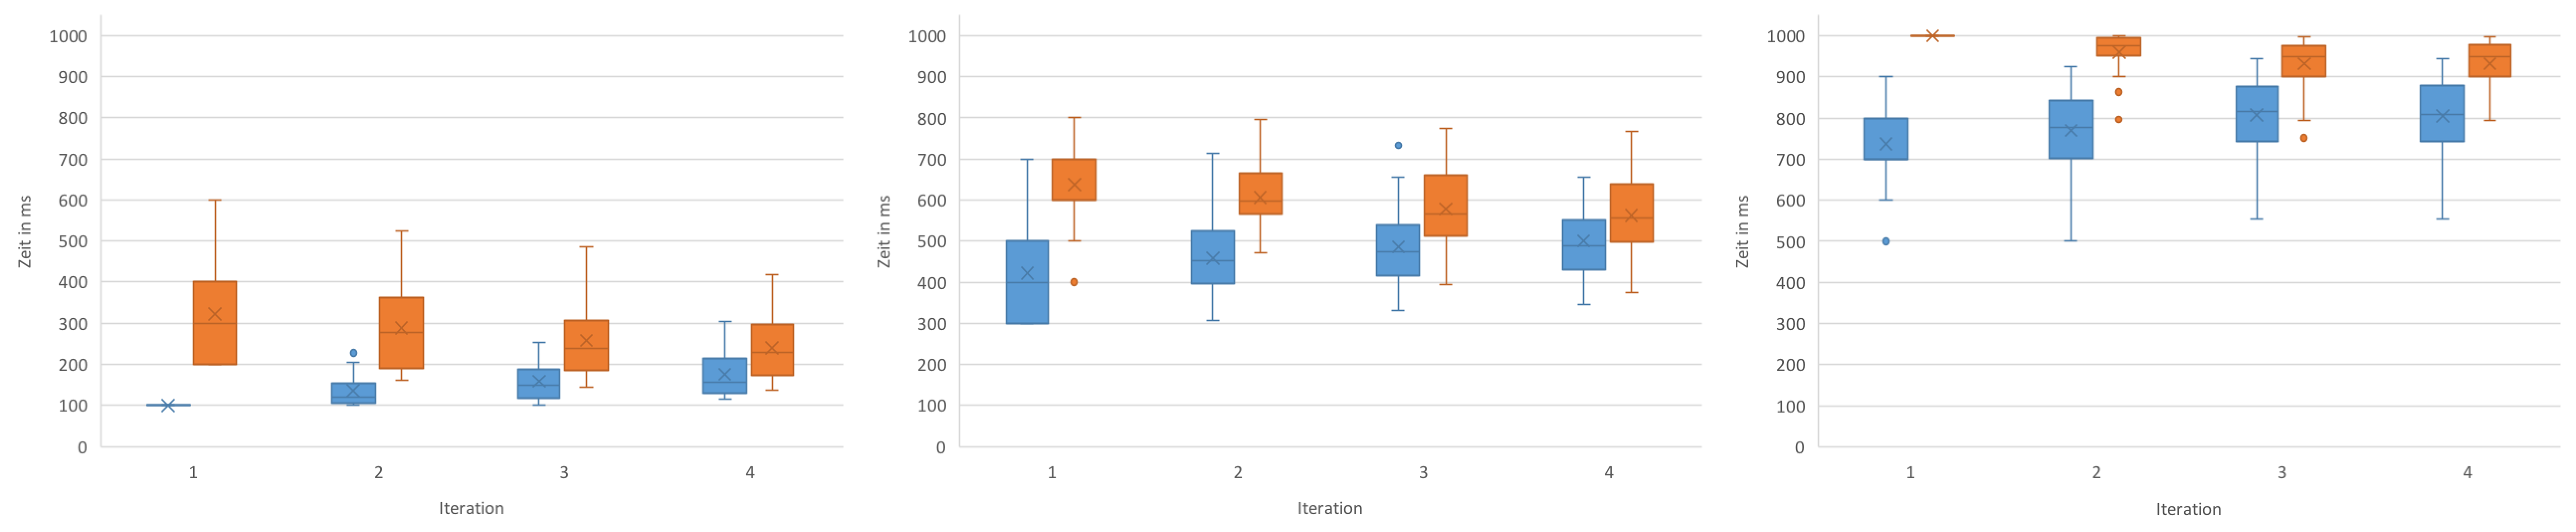
\includegraphics[width=\textwidth]{pics/analyse/algo/MinMax/MinMaxFinal.png}
%	\caption{Darstellung des Minimum (in blau) und Maximum (in rot) im Verlauf der 4 Iterationen des Algorithmus. Das erste Bild zeit Kurz, gefolgt von Mittel und Lang.}
%	\label{fig:MinMaxSignale}
%\end{figure}

Der Algorithmus wurde insgesamt vier mal ausgef{\"u}hrt, anschlie{\ss}end wurde aus der letzten Population der personalisierte Wert gemittelt. 

\paragraph{Kurz}
Eine der gr{\"o}{\ss}ten Ver{\"a}nderungen im Diagramm \autoref{MinMaxSignale} gibt es bei \textbf{Kurz}; die oberste Grenze vom Maximum ist nach vier Iterationen von 600ms auf 415ms gesunken. 
Die obere Grenze des Minimum ist von 100ms auf 300ms gestiegen. 
%Der Bereich verkleinert insgesamt das Intervall um 44\% von 100 bis 600ms auf 140 bis 420 ms. 
Der Median von den Maximum und Minimum konvergieren in die gleiche Richtung. 
Nach vier Iterationen ist der Median vom Minimum um 80ms nach oben und der Median von dem Maximum auch um 80ms nach unten gewandert. 
Das Minimum und Maximum {\"u}berschneidet sich in der 2. Iteration nur minimal. 
In der 4. Iteration {\"u}berschneiden sich Minimum und Maximum um 150ms. 
Das 50\% Quartil vom Minimum w{\"a}chst um bis zu 100ms, wobei das 50\% Quartil beim Maximum von einem 200ms Intervall auf ein 120ms Intervall verkleinert. 
Das gesamte Intervall von \textit{Kurz} verkleinert sich insgesamt um 44\% von 100-600ms auf 140-420ms, somit ist das die gr{\"o}{\ss}te Ver{\"a}nderung unter allen Intervallen.



\paragraph{Mittel}
In der ersten Iteration besitzt man schon {\"u}berschneidungen des Minimum und Maximum. 
Von der ersten zur zweiter Iteration verschieben sich die Grenzen des Minimum um ca. 10 ms nach oben, diese werden im Verlauf der Iteration minimal kleiner.  
Die Grenzen des Maximums hingegen werden gr{\"o}{\ss}er und verschieben sich anschlie{\ss}end minimal nach unten. 
Das 50\% Quartil verkleinert sich um 40\% sich beim Minimum von einem 200ms Intervall auf ein 120ms Intervall und verschiebt sich anschlie{\ss}end im Verlauf der folgenden Iterationen nur nach oben. 
Bei \textit{Mittel} habt sich das gesamt Intervall um 16\% von 300-800ms auf 345-766ms verkleinert.


\paragraph{Lang}
Die meisten Ausrei{\ss}er sind in bei Lang vertreten, hier hat man in der zweiten Iteration schon ein Maximum von 1000ms auf unter 800ms und 880ms erhalten, das ist eine {\"a}nderung eines Maximums um 200ms nach nur einer Iteration bei einem Probanden.
Die 50\% Quartile des Maximums werden Minimal gr{\"o}{\ss}er und wachsen nach unten.
Das 50\% Quartile des Minimums werden die kurzzeitig gr{\"o}{\ss}er, minimiert sich minimal wieder im Verlauf.
Die Grenzen des gesamten Intervalls von \textit{Lang} haben sich um 11\% von 500-1000ms auf 555-997ms minimiert.
Zwischen der 3. und 4. Iteration bei \textit{Lang} ist es das einzige mal vorgekommen, dass zwischen zwei Itterationen bis auf 3ms keine Unterschiede erkennbar sind.
Das w{\"u}rde bedeuten, dass nach der 3. Generation f{\"u}r die Probanden schon ein sehr gut unterscheidbares Ergebnis vorhanden gewesen ist.
% {\"a}ndern sich aber wieder auf mit dem Ausrei{\ss}er der ersten Iteration auf das gleiche Intervall und verschieben sich pro Iteration leicht nach oben.

%\\

Unter den Signaltypen {\"u}berschneiden sich die Iterationen die Grenzen selbst zwischen den Iterationen selbst. 
Diese {\"U}berschneidungen verringern sich nach den 4 Iterationen.

Das Minimum steigt stetig und das Maximum verringert sich. 
Denn genau diesen Effekt wollte man auch erzielen, dass der Benutzer zu seinen personalisierten Wert konvergiert.
Bei Kurz und Mittel {\"u}berschneiden sich die 50\% Quartile. 
Bei Lang {\"u}berschneiden diese in keiner Iteration.

Schlussfolgernd kann man sagen, dass die man anhand der 50\% Quartile vom Maximum und Minimum aller Probanden einen Kurzes Signal in dem Bereich von 130ms bis 300ms, ein Mittleres Signal zwischen 430ms und 640ms und ein Langes Signal zwischen 740ms und 980ms die gebildet haben. 




\paragraph{Grenzen nach dem Algorithmus}

\begin{figure}[htbp] 
            \centering
   	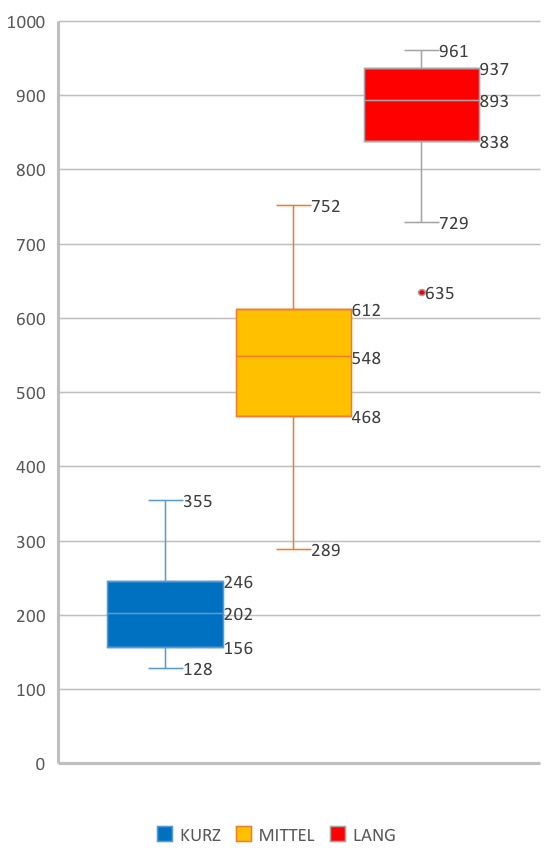
\includegraphics[width=0.8\textwidth]{pics/analyse/algo/MinMax/GrenzenNachAlgo.png}
	\caption{Nach der Vierten Iteration gemittelte personalisierte Werte in ms}
	\label{fig:GrenzenNachAlgo}
\end{figure}

In dem Diagramm \autoref{fig:GrenzenNachAlgo} sind alle gemittelten personalisierten Werte nach der vierten Iteration abgebildet. 
Daraus l{\"a}sst sich ableiten, dass zwischen den Signaltypen von \textit{Kurz}, \textit{Mittel} und \textit{Lang} sich die Grenzen {\"u}berschneiden und man somit sagen kann, dass man diese Bereiche auf f{\"u}r vordefinierte Signale meiden sollte. 
Die Grenzen {\"u}berschneiden zwischen \textit{Kurz} und \textit{Mittel} von 289-355ms und zwischen \textit{Mittel} und \textit{Lang} von 729-752ms.
F{\"u}r die einzelnen Signaltypen hat sich der Median f{\"u}r \textit{Kurz} bei 202ms, f{\"u}r \textit{Mittel} bei 548ms und \textit{Lang} bei 893ms bestimmen k{\"o}nnen.
Die oberen 25\% von \textit{Lang} und die unteren 25\% von \textit{Kurz} weisen nur eine minimale Abweichung auf. 
Im Gegensatz dazu gibt es eine Abweichung von genau 109ms bei den oberen 25\% von \textit{Kurz} und den unteren 25\% von \textit{Lang}.
Es gibt einen Ausrei{\ss}er bei \textit{Lang} mit einem Wert von 635ms, dabei handelt es sich nicht um keinen Fehler, sondern einen Probanden der genau dies f{\"u}r sich als personalisierten Wert bestimmt hat.
Im Vergleich der inneren 50\% von den jeweiligen Signaltypen wei{\ss}t \textit{Kurz} einen Intervall von 90 ms und \textit{Lang} einen Intervall von 99ms auf, wobei \textit{Mittel} diesen Wert von 144 ms am gr{\"o}{\ss}ten Bereich ist und um nahezu 50ms gr{\"o}{\ss}er als Kurz und Lang ist. 


\paragraph{Stimmung im Verlauf des Algorithmus}

\begin{figure}[htbp] 
            \centering
   	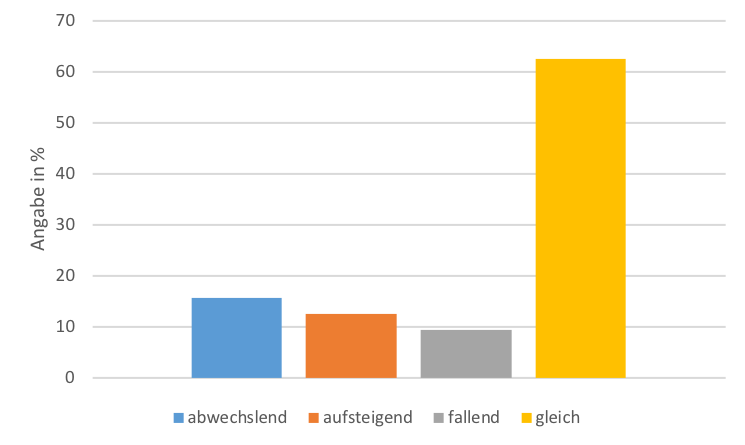
\includegraphics[width=0.8\textwidth]{pics/analyse/person/Stimmung.png}
	\caption{Bewertung der Stimmung}
	\label{fig:Stimmung}
\end{figure}

Nach jeder Iteration wurden die Benutzer gefragt, wie Ihre Stimmung \autoref{fig:Stimmung} aktuell sei. 
Dabei hat es bei 62\% aller Probanden keine {\"A}nderung der Stimmung gegeben. 
Diese Probanden hatten Ihre Stimmung mit \textit{Gut} oder \textit{Sehr gut} bewertet gehabt. 
Im Gegensatz dazu hat sich die Stimmung bei 16\% der Probanden entweder zwischen \textbf{Gut} und \textbf{Sehr gut} oder \textbf{Gut} und \textbf{OK} abgewechselt. 
Des Weiteren gab es bei 13\% der Probanden eine aufsteigende Stimmung und bei den restlichen 9\% ist die Stimmung pro Iteration gefallen.

Somit kann man feststellen, dass die Anzahl von vier Iterationen keinen wirklichen Einfluss auf die Stimmung des Benutzers ausgewirkt hat.

% die ben{\"o}tigt wurde um den Algorithmus auszuf{\"u}hren, sich nicht auf die Stimmung Stimmung sich nicht  ausgewirkt hat. 

\paragraph{Replays eines Signals}

\begin{figure}[htbp] 
            \centering
   	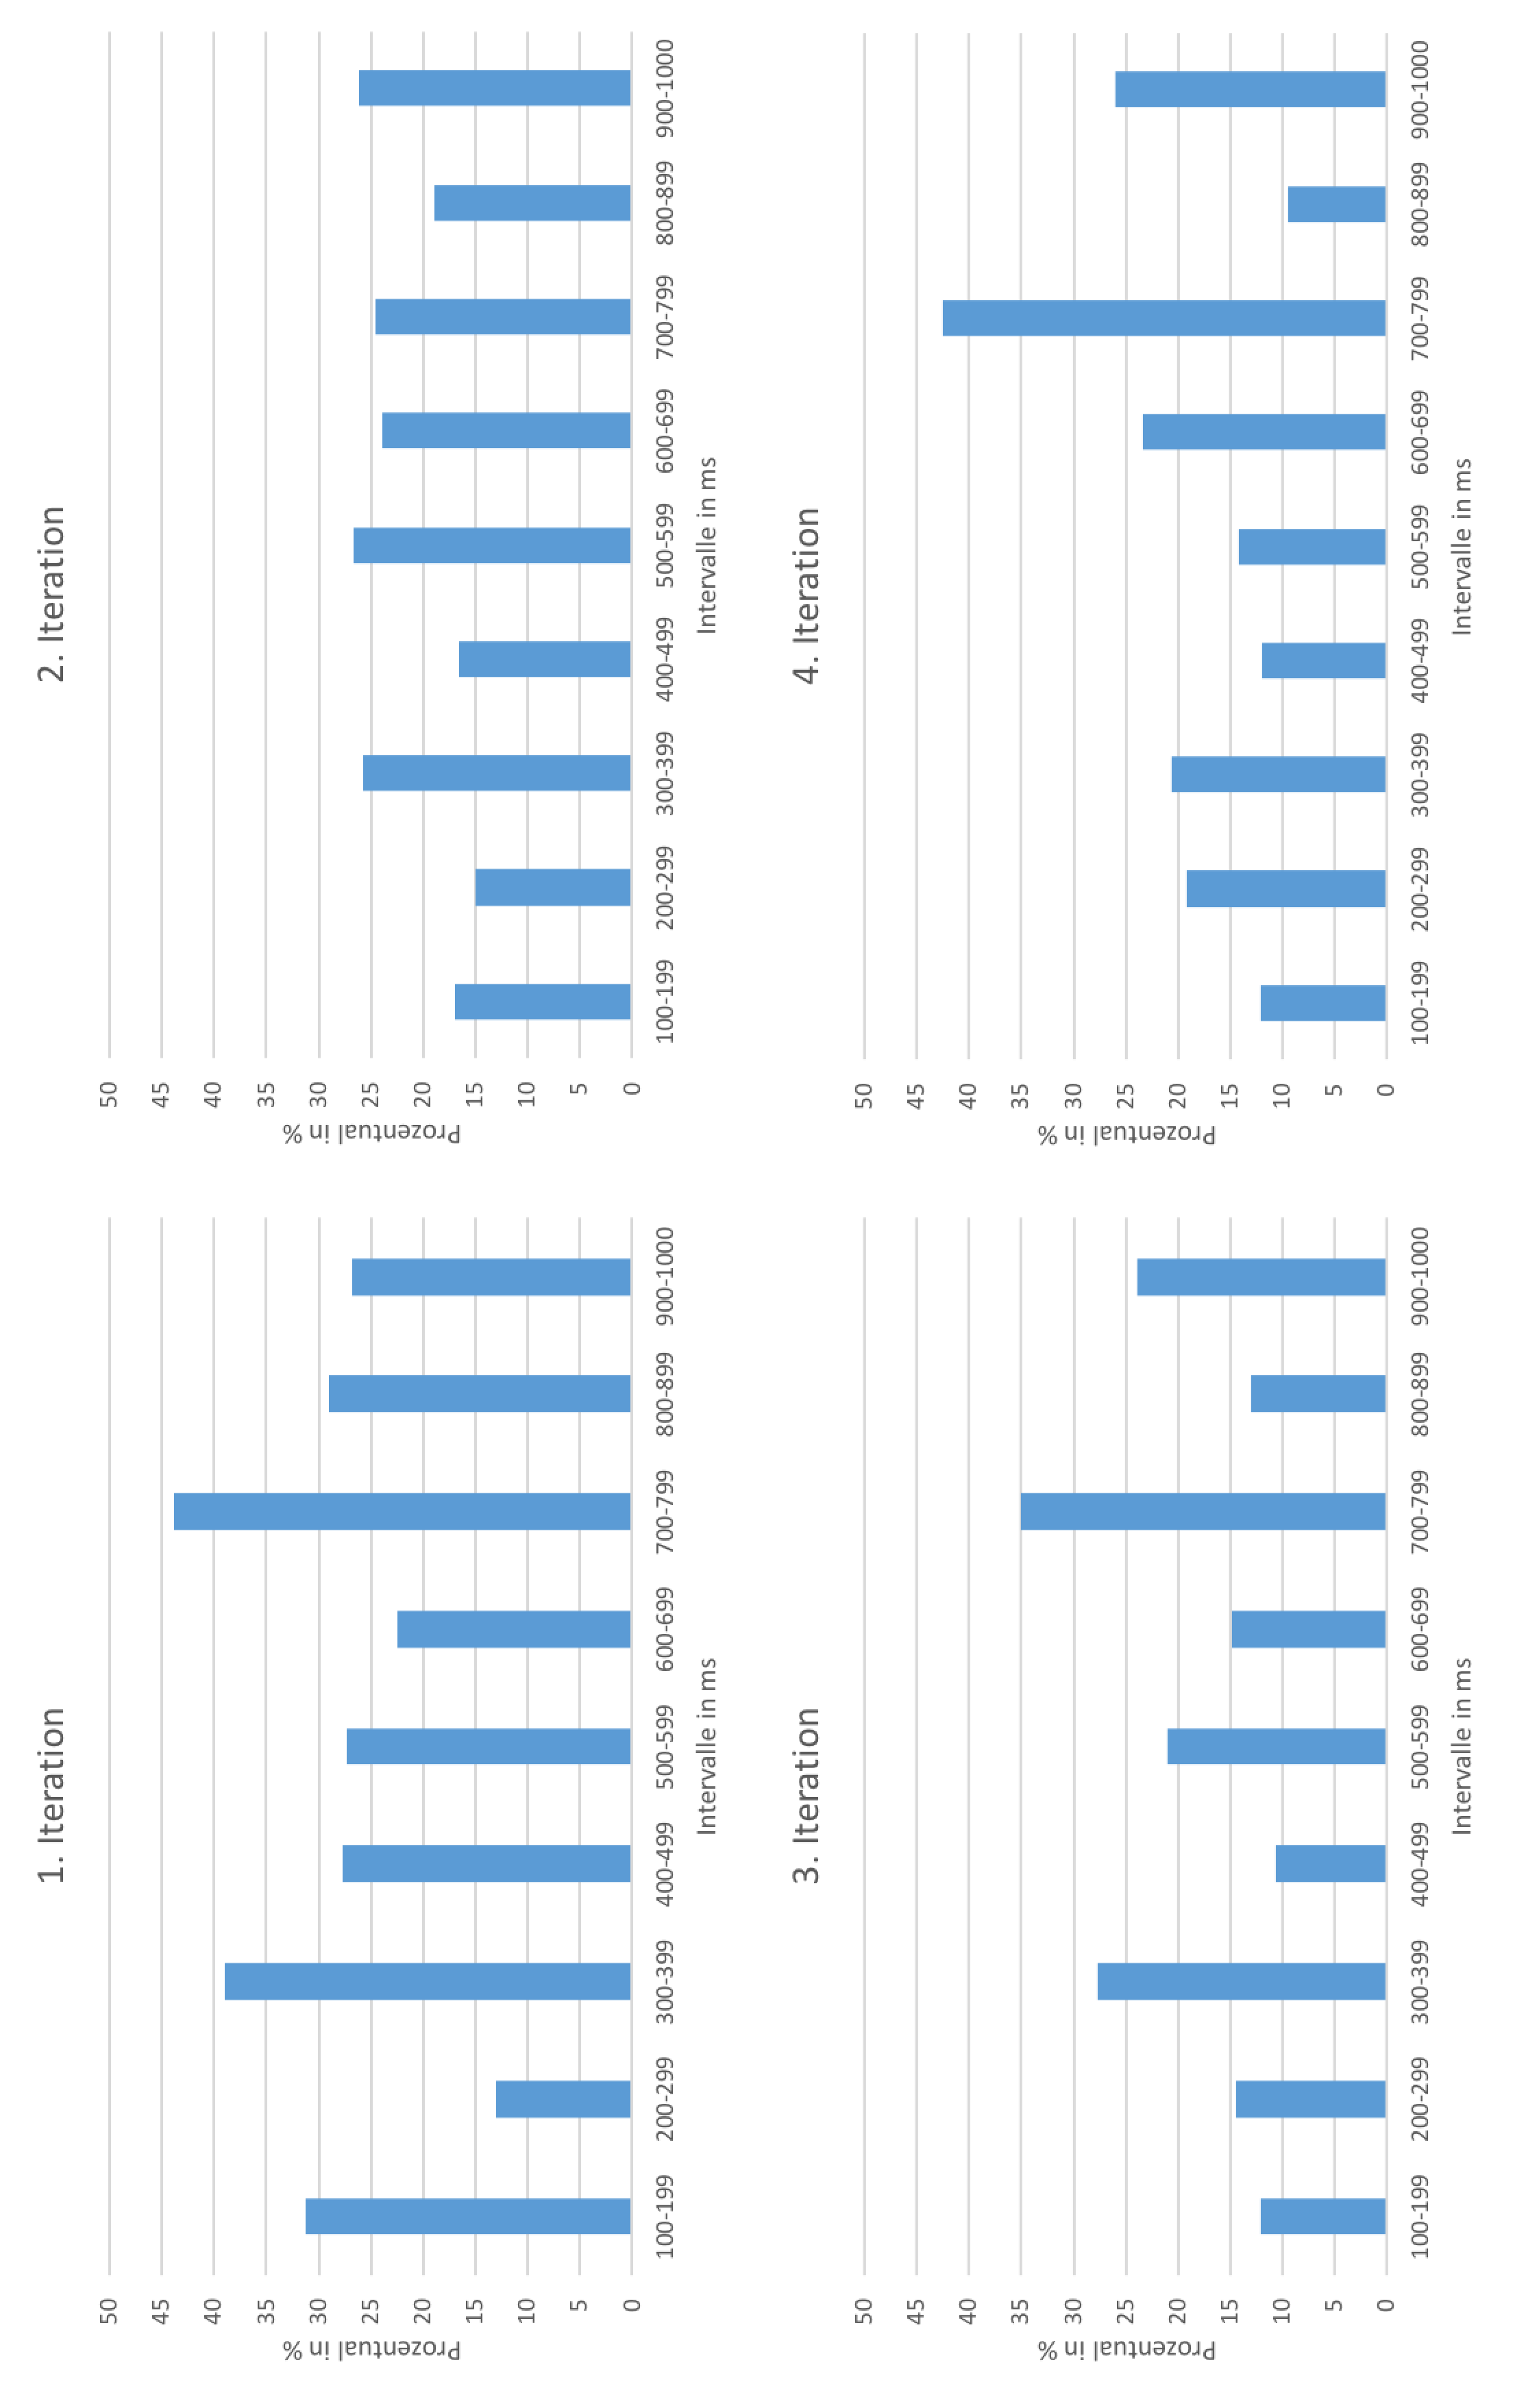
\includegraphics[width=\textwidth]{pics/analyse/algo/Replay/ReplayFinal290.png}
	\caption{Anzahl der Replays innerhalb von Zeitintervallen {\"u}ber dem Verlauf des Algorithmus}
	\label{fig:ReplayFinal290}
\end{figure}

Man hat dem Probanden die M{\"o}glichkeit geboten, ein Signal wiederholen zu d{\"u}rfen. 
Im Verlauf des Algorithmus wollte man herausfinden wie oft unter allen Probanden auf Replay f{\"u}r ein bestimmtes Intervall Replay gedr{\"u}ckt wurde \autoref{fig:ReplayFinal290}. 
%Die Anzahl der wie oft auf Replay gedr{\"u}ckt wurde 

In der ersten Iteration haben 44\% der Probanden in dem Intervall von 700-799ms die gr{\"o}{\ss}ten Schwierigkeiten gehabt ein Signal zuzuordnen und sich das Signal erneut abgespielt. 
Der Bereich, der am wenigsten wiederholt abgespielt werden musste war 200-299ms. 
Die Restlichen Intervalle der ersten Iteration wurden mit einem Mittelwert von 32\% erneut abgespielt.

In der zweiten Iteration hat sich die Anzahl der Replays um einiges verringert, hier war der Mittelwert insgesamt bei 22\%, das Minimum war bei 200-299ms im Wert von 15\% und das Maximum bei 500-599ms mit 27\%.  
Die dritte Iteration hat eine Verbesserung bei allen nahezu allen Werten gehabt, bis auf das Intervall von 700-799ms was auf 35\% angestiegen ist; insgesamt ist der Mittelwert in dieser Iteration bei 19\%. 

Selbst in der letzten Iteration hat sich ein globales Minimum unter allen Iterationen bei 800-899ms von 9,5\% gebildet. Der globale Maximum war bei 700-799ms in der ersten Iteration mit 43\%, ist aber auch in der vierten Iteration, trotz Verbesserungen zwischen durch das Maximum mit 42,5\%. 

Man kann daraus erkennen, dass die Probanden genau an dem Bereich von Kurz zu Mittel, was sich in der 4. Iteration bei 200-399ms bewegt, und Mittel zu Lang, dass zwischen 600-799ms liegt, am meisten den Replay Knopf gedr{\"u}ckt haben. 
Ein viertel aller Probanden haben bei 900-1000ms in jeder Iteration das Signal erneut abgespielt. 
Jedoch kann man in der vierten Iteration sehr gut erkennen, dass die Signale mit den Werten 100-199ms, 400-599ms und 800-899ms am geringsten erneut abgespielt werden mussten.
Im Durchschnitt wurde, der Replay Button 1,7mal gedr{\"u}ckt, wenn man ein Signal erneut abgespielt haben wollte. 
Dabei war das Minimum einmal und das Maximum neun mal, dass man das Signal erneut abgespielt hat.

\paragraph{Mittelwert}
Beim Verlauf des Algorithmus konnte man feststellen, dass zwischen der ersten und der letzten Iteration unter allen Probanden der Mittelwert sich wie im folgenden Verhalten hat. 
\textit{Kurz} hatte eine durchschnittliche Abweigung von 10,11\% bei einem Minimum von 1\% und einem Maximum von 23\%. 
Weiterhin habe sich der Mittelwert bei den beiden Signaltypen \textit{Miitel} und \textit{Lang} von der ersten zur letzten Iteration im Durchschnitt nur um 3,34\% ver{\"a}ndert.
Dabei war das Minimum bei 0,09\% und ein Maximum bei 9,9\% f{\"u}r \textit{Mittel} sowie ein Minimum von 0,06\% und ein Maximum von 15,33\% f{\"u}r \textit{Lang} vorhanden.

\paragraph{Beantwortung der Fragen}
\begin{figure}[htbp] 
            \centering
   	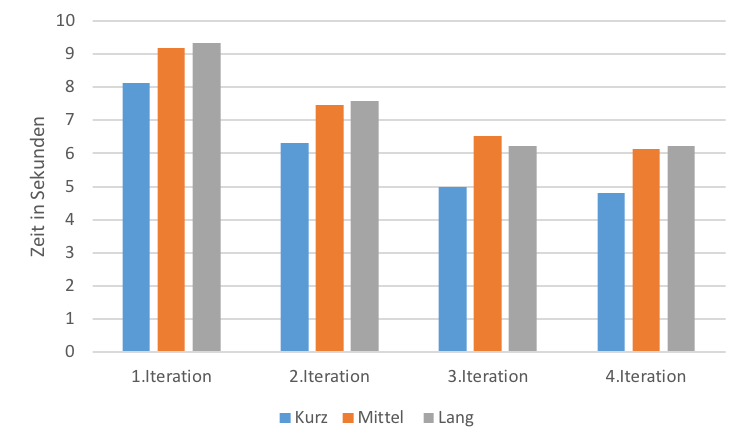
\includegraphics[width=0.8\textwidth]{pics/analyse/algo/ZeitDurchschnitt.png}
	\caption{Durchschnittlich ben{\"o}tigte Zeit der Probanden, um die drei Fragen des Algorithmus zu bewerten.}
	\label{fig:ZeitDurchschnitt}
\end{figure}
Im Verlauf des Algorithmus hat man auch die Zeit \autoref{fig:ZeitDurchschnitt}, die ben{\"o}tigt wurde um die Fragen f{\"u}r ein Signal zu beantworten, gespcierht. 
Daraus hat sich ergeben, dass \textit{Kurz} in jeder Iteration um einer ganzen Sekunde schneller beantwortet wurde. 
F{\"u}r \textit{Mittel} und \textit{Lang} hat man im Durchschnitt immer gleich viel Zeit ben{\"o}tigt.
Nach der dritten Iteration ist der Wert f{\"u}r alle drei Signaltypen nahezu konstant geblieben, desweiteren hat sich bis zur dritten Iteration bei allen Signaltypen der Wer um drei Sekunden verringert. 
Daraus l{\"a}sst sich ableite, dass die Probanden sich an die Signale gew{\"o}hnt haben und die drei Fragen schneller beantworten konnten.

\paragraph{Verlauf der Werte}
\begin{figure}[htbp] 
            \centering
   	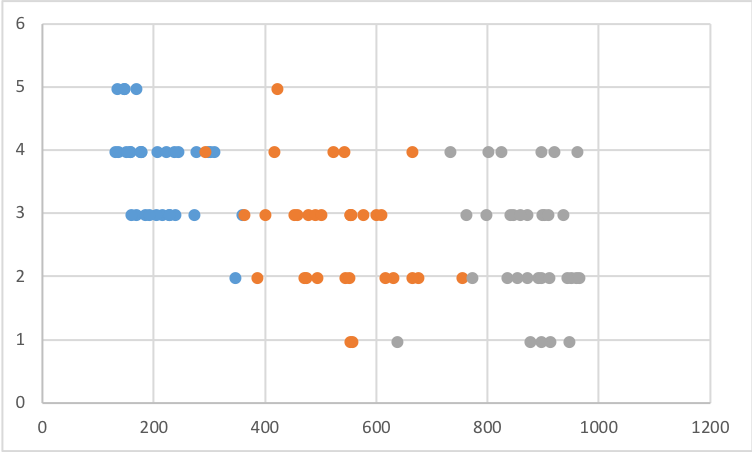
\includegraphics[width=0.8\textwidth]{pics/analyse/algo/ergebnisnachAlgo.png}
	\caption{Personalisierte Werte der einzelnen Probanden, die in dem Diagramm der St{\"a}rke {\"u}ber die Zeit dargestellt werden.}
	\label{fig:ergebnisNachAlgo}
\end{figure}

Anhand des Diagramms \autoref{fig:ergebnisNachAlgo} kann man erkennen, dass die meisten Probanden ein st{\"a}rkeres \textit{Kurz} Signal sowie ein schw{\"a}cheres \textit{Lang} Signal bevorzugt haben. F{\"u}r das Signal \textit{Mittel} hat man sich jedoch in dem mittleren St{\"a}rkebereich befunden.

\begin{figure}[htbp] 
            \centering
   	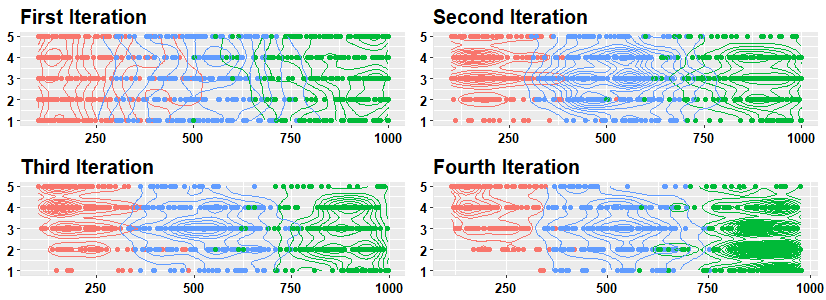
\includegraphics[width=\textwidth]{pics/analyse/algo/gruppierung.png}
	\caption{Darstellung der St{\"a}rke zu der jeweiligen Signall{\"a}nge {\"u}ber dem Verlauf des Algorithmus. Dabei bildet rot \textit{Kurz}, blau \textit{Mittel} und gr{\"u}n \textit{Lang} ab.}
	\label{fig:gruppierung}
\end{figure}

In der ersten Itteration \autoref{fig:gruppierung} sieht man sehr sch{\"o}n, wie es noch keine wirklliche Unterteilung existiert, es gibt die Bereiche bis 250ms in denen sich das Signal \textit{Kurz} befindet und von 800-1000ms auch \textit{Lang}, aber es gab {\"u}berschneidungen in den Bereich von \textit{Mittel} mit den anderen beiden Signaltypen. 
Anhand der zweiten Iteration haben sich schon leichte Cluster gebildet, bei denen es dennoch Ausrei{\ss}er von Kurz und Mittel an den Werten nahe 500ms existieren. 
Bis zur vierten Iteration verdichten sich die Signale von \textit{Kurz} in dem oberen linken Bereich, das bedeutet, dass man f{\"u}r Signale vom Typ \textit{Kurz} eher st{\"a}rkere Signale bevorzugt hat. 
Die Signale des Typs \textit{Mittel} haben im Verlauf des Algorithmus genau in der Mitte bei dem Wert 500ms und der mittleren St{\"a}rkestufe eine Hochpunkt gebildet. 
Desweiteren hat sich das Signaltyp \textit{Lang} in den St{\"a}rkestufen eins (f{\"u}r sehr schwach) bis drei (f{\"u}r o.k.) einzelne Cluster gebildet. 
Wohingegen bei \textit{Kurz} und \textit{Mittel} sich ein Hochpunkt gebildet haben, hat sich bei \textit{Lang} f{\"u}r die St{\"a}rkestufen eins (f{\"u}r sehr schwach) bis drei (f{\"u}r o.k.) jeweils ein Cluster gebildet.

Man kann zweifellos erkennen, dass wenn man noch weitere Iterationen ausgef{\"u}hrt h{\"a}tte, w{\"u}rde sich das Ergebnis weiter in einem Punkt verdichten. 

%H{\"a}tte man noch mehr Iterationen des Algorithmus ausgef{\"u}hrt, w{\"a}re es zweifellos, dass sich das Ergebnis weiter in einem Punkt verdichten w{\"u}rden. 


\paragraph{Muster}

\begin{table}[]
\centering
\caption{Durchschnittliche Genauigkeit zur Erkennung eines Signals der Probanden {\"u}ber die Kategorien (Angaben in \%)}
\label{MusterGenauigkeit}
\begin{tabular}{lll|lll|l}
%\hline
\multicolumn{3}{l}{Genetisch} & \multicolumn{3}{|l|}{Generisch} & Kategorie      \\ \hline
3er    & 4er    & 5er   & 3er    & 4er    & 5er   &                             \\ \hline
81     & 77     & 75    & 76     & 69     & 66    & {\"u}ber alle Probanden         \\ \hline
76     & 71     & 74    & 75     & 67     & 63    & weiblich                    \\
83     & 79     & 77    & 80     & 74     & 71    & m{\"a}nnlich                    \\ \hline
80     & 74     & 77    & 79     & 74     & 71    & musikalisch                 \\
80     & 75     & 72    & 77     & 69     & 66    & nicht musikalisch           \\ \hline
81     & 76     & 75    & 78     & 72     & 70    & spielen Spiele              \\
75     & 70     & 70    & 74     & 63     & 58    & spielen keine Spiele        \\ \hline
86     & 84     & 80    & 83     & 79     & 75    & nutzten Smartwatch          \\
78     & 72     & 72    & 76     & 68     & 66    & nutzten keine Smartwatch    \\ \hline
83     & 78     & 73    & 80     & 70     & 67    & nutzten Taktiles Ger{\"a}t      \\
76     & 72     & 75    & 75     & 70     & 69    & nutzten kein Taktiles Ger{\"a}t
\end{tabular}
\end{table}

Die Tabelle \autoref{MusterGenauigkeit} beschreibt, wie genau die Probanden ein Signal aus den Mustern erkennen konnten, man hat die generischen Muster mit den genetischen Mustern verglichen, sowie f{\"u}r jede Gruppierung von Probanden die Auswertung neu bestimmt. 
%Die Tabelle \autoref{MusterGenauigkeit} beschreibt, wie genau die Probanden ein Muster ohne Fehler erkennen konnten, man hat die generischen Muster mit den genetischen Mustern verglichen, sowie f{\"u}r jede Gruppierung von Probanden die Auswertung neu bestimmt. 
%Dabei hat man in den jeweiligen Kategorien nach den gelisteten Kategorien die Genauigkeit gruppiert.

Laut der Tabelle kann man feststellen, dass die Probanden die keine Computerspiele spielen, die einzelnen Signale der generischen f{\"u}nfer Muster nur zu 58\% richtig erkannt haben. Dieser Wert ist das Globale Minimum unter allen Gruppierungen der Probanden.
Bei den Probanden, die schon einmal eine Smartwatch nutzten, haben bei den genetischen dreier Mustern ein einzelnes Signal mit 86\% Wahrscheinlichkeit richtig erkannt, der auch als globales Maximum unter allen Probanden-Gruppen existiert.

%Das Globale Maximum ein Signal richtig zu erkennen, war bei den genetischen Mustern mit drei Signalen, bei einem Wert von 86\% durchschnittlicher Genauigkeit bei Probanden, die schon mal eine Smartwatch benutzt hatten. 
%Das Globale Maximum war bei den genetischen Mustern mit drei Signalen bei einem Wert von 86\% durchschnittlicher Genauigkeit bei Probanden, die schon mal eine Smartwatch benutzt hatten. 
%Das Globale Minimum war bei der Gruppe an Probanden die keine Computerspiele spielen und zwar mit der Genauigkeit von 58\% bei generischen Mustern mit 5 Signalen.

Unter den vorliedenden Ergebnissen, haben die m{\"a}nnlichen Probanden im Vergleich zu den weiblichen Probanden die einzelnen Signale unter allen Muster-Typen besser erkannt.
%Unter den vorliegenden Ergebnissen, waren die m{\"a}nnlichen Probanden bei der Erkennung von komplett richtigen Mustern im Durchschnitt immer um einige Prozent besser.
Die musikalischen und nicht musikalischen Probanden erkennen bei den dreier Mustern die Signale gleich gut, wobei bei den vierer und f{\"u}nfer Muster die musikalischen Probanden bis zu 5\% besser waren.
Bei den dreier Mustern k{\"o}nnen die musikalischen im Vergleich zu nicht musikalischen Probanden die Signale gleich gut erkennen, jedoch zeigen die musikalichen Probanden bei vierer und f{\"u}nfer Muster eine Verbesserung bis zu 5\%.
%Unter der Kategorie "`musikalisch"' kann man nachvolzeihen, dass bei den dreier Mustern die Signale gleichgut erkannt worden sind. 
%Bei den Musikalischen Probanden sind bei den genetischen dreier Mustern gleich gut wie die nicht musikalischen Probanden. 
%Bei den vierer und f{\"u}nfer Signalen waren die musikalischen Probanden jedoch um bis zu 5\% besser.
Allgemein k{\"o}nnen die gelegendlich Computerspiele spielenden Probande im Gegensatz zu nicht-Spielern alle abgespielten Signale der Muster-Typen besser zuweisen. Wenn wir ins Detail gehen, liegt bei den generischen f{\"u}nfer Muster die Abweichung von 12\%.
%Die Probanden die gelegendlich Computerspiele spielen, haben die Signale aller Muster-Typen besser erkannt, als die Probanden die keine Computerspiele gespielt haben, hier lag der gr{\"o}{\ss}te Unterschied n{\"a}mlich bei den generischen f{\"u}nfer Muster, die eine Abweichung von 12\% aufweisen.
%Die Probanden die gelegendlich Computerspiele spielen haben die Muster im Durchschnitt genauer erkannt als die Probanden die keine Computer spiele gespielt haben, hier lag der gr{\"o}{\ss}te Unterschied n{\"a}mlich bei den generischen f{\"u}nfer Muster, die eine Abweichung von 13 \% aufweisen.
Dasselbe Ergebnis, n{\"a}mlich 12\% Unterschied kommt bei Probanden vor, die schon mal eine Smartwatch getragen haben.
%Das selbe gilt f{\"u}r die Probanden, die schon mal eine Smartwatch benutzt haben, hier lag der Unterschied bei 12 \%.

Bei der letzten Gruppe wird es interessant, denn hier haben genau 50\% der Probanden schon mal ein Taktiles Ger{\"a}t verwendet. 
Dabei wurde um 8\% der Signale der genetischen dreier Muster sowie um 4\% der generischen Muster von den Teilnehmern, die Erfahrung mit den taktilen Ger{\"a}ten hatten, besser erkannt.
%Dabei wurden die Signale der genetischen dreier Muster um 8\% und bei den generischen Mustern um 4\% besser erkannt.
%Diese waren bei den genetischen dreier Mustern um 8\% besser erkannt und die generischen um nur 4\%. 
Bei den Signalen der f{\"u}nfer Muster haben die Probanden, die schon einmal ein Taktiles Ger{\"a}t verwendet haben, die Signale um 2\% besser erkannt.
%Bei den f{\"u}nfer Mustern haben Probanden, die schon mal ein Taktiles Ger{\"a}t verwendet haben die Signale um 2\% besser erkannt. 

Im Vergleich zu den generischen Muster wurden die Signale der genetischen Muster {\"o}fter richtig zuge{\"o}rdnet. 
Die Genauigkeit erreichte sogar bei dem genetischen dreier Muster bis zu 82\%. 
Somit ist es um 5\% besser als der Wert von der generischen dreier Muster.
%Im Vergleich der genetischen und generischen Muster aller Probanden, wurden die Genetischen Signale eindeutig {\"o}fter richtig erkannt als die generischen Werte. 
%Die genetischen dreier Muster wurden die Signale mit 82\% um 5\% besser erkannt als die generischen dreier Muster. 
Obwohl der Prozenzsatz bei den vierer Mustern ingesamt gesunken ist, gewinnt jedoch der Unterschied an Ausdehnung.
Hier erh{\"o}ht sich das Optimierungspotenzial bei genetischen vierer Mustern um 8\%.
%Bei den vierer Mustern ist der Prozenzsatz insgesamt weiter herunter gegangen, jedoch ist der Unterschied gr{\"o}{\ss}er geworden und zwar ist es auf 77\% bei den genetischen vierer Mustern im Vergleich eine Verbesserung von 8\% zum generischen. 
Generell wurden 75\% der Signale bei den genetischen f{\"u}nfer Mustern korrekt erkannt und somit wird nur zwei drittel der Signale von den generischen f{\"u}nfer Mustern als richtig empfunden.
%Bei den f{\"u}nfer Signalen wurden drei von vier Signale (75\%) korrekt erkannt. 
%Bei den generischen f{\"u}nfer Mustern wurden nur zwei von drei Signalen richtig erkannt. \\

%Unter Betrachtung der genetischen und generischen Muster, gibt es bei den dreier Mustern eine minimale Abweichung von 0\% bis zu einem Maximum von 5\%, in denen die genetischen Muster besser erkannt worden sind als die generischen. 
%Bei den 4er Muster sieht es {\"a}hnlich aus, mit einem Minimum von 0\% und einem Maximum von 8\% Abweichung. 
%Bei den 5er Mustern hat man eine Abweichung von 4\% bis zu 12\%. 


%Die Auswertung meiner Daten haben ergeben, dass musikalische Probanden 


\begin{figure}[htbp] 
	\centering
	\begin{minipage}[t]{0.8\textwidth}
		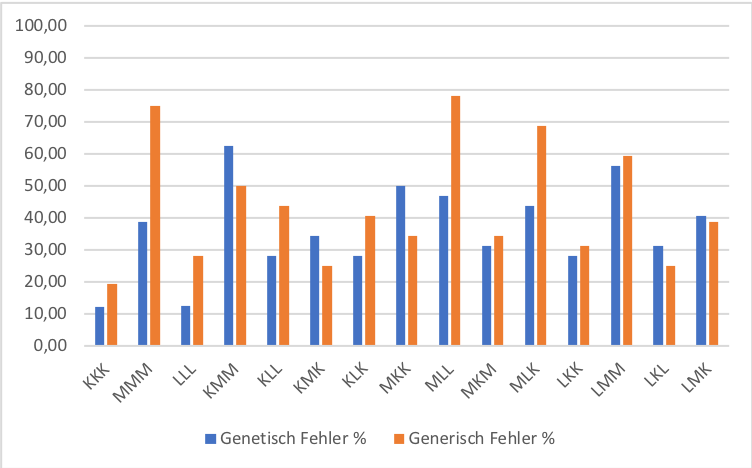
\includegraphics[width=\textwidth]{pics/analyse/algo/ohneFehler/Fehler3.png}
	\end{minipage}
	\begin{minipage}[t]{0.8\textwidth}
		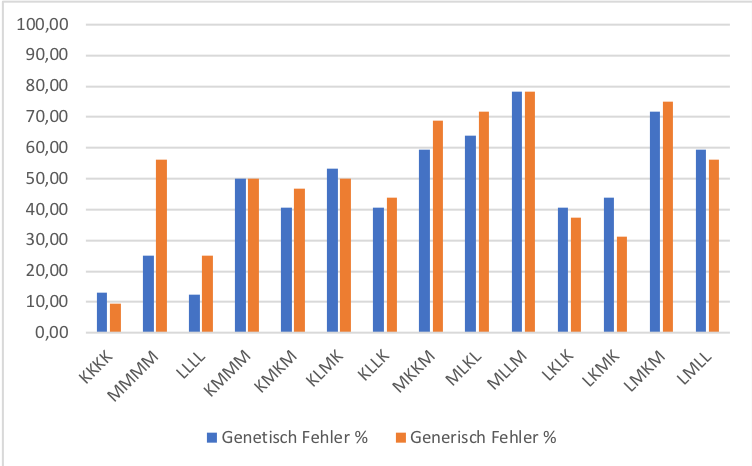
\includegraphics[width=\textwidth]{pics/analyse/algo/ohneFehler/Fehler4.png}
	\end{minipage}
	\begin{minipage}[t]{0.8\textwidth}
		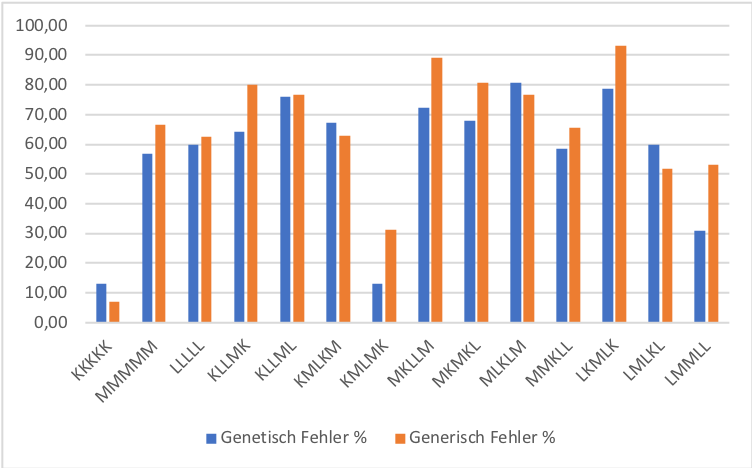
\includegraphics[width=\textwidth]{pics/analyse/algo/ohneFehler/Fehler5.png}
	\end{minipage}
	\caption{Anhand der Diagramme wird die H{\"a}ufigkeit, wie oft einem Muster nicht richtig erkannt worden ist. Es z{\"a}hlt ein Muster als nicht erkannt, wenn mindestens ein Signal nicht korrekt zugrordnet werden konnte.   
	%Darstellung der Wahrscheinlichkeit {\"u}ber alle Probanden, wie oft bei einem Muster mindestens ein Signal nicht korrekt zugeordnet werden konnte.
	Dabei wurden die genetischen und generischen Fehlerangaben (in \%) direkt miteinander verglichen. 
	Die Diagramme wurden f{\"u}r die jeweiligen Muster (dreier, vierer und f{\"u}nfer) seperat angezeigt.
	Hier steht K f{\"u}r \textit{Kurz}, M f{\"u}r \textit{Mittel} und L f{\"u}r \textit{Lang}}
	\label{fig:FehlerBild}
\end{figure}
 
In der Darstellung \autoref{fig:FehlerBild} wurden die Muster und die H{\"a}ufigkeit, wie oft die Probanden das Muster nicht als solches erkannt haben, dargestellt. 
Die Muster \textit{KKK} und \textit{LLL} haben die meisten Probanden korrekt erkannt, nur 12 \% haben bei den genetischen Werten das Signal nicht korrekt erkennen k{\"o}nnen. 
Au{\ss}erdem wurden hat man bei den selben Mustern mit den generischen Werten eine Verschlechterung von 7\% bei \textit{KKK} und eine Verdopplung bei \textit{LLL} festgestellt, wobei man das gleiche Verhalten auch bei den vierer Muster erkennen kann.

Im Vergleich der drei Diagramme kann man erkennen, dass f{\"u}r die dreier und vierer Muster mit nur einem Signaltypen bei \textit{Kurz} und \textit{Lang} nahezu identisch sind und die genetischen Muster {\"o}fter erkannt wurden als die generischen Muster. 
Das Muster mit durchgehenden \textit{Mittel} Signalen haben die Probanden bei den dreier sowie bei den vierer Mustern jeweils das genetische bevorzugt, da die generischen Muster um jeweils das Doppelte schlechter erkannt wurde. 

Unter allen dreier Mustern wurden zwei drittel der genetischen Muster besser als die generischen Muster erkannt. 
Zus{\"a}tzlich befindet sich der Durschnitt bei 36\% f{\"u}r die genetischen und bei 43\% f{\"u}r die generischen dreier Muster.
Dieser Prozenzssatz steigt bei den genetischen vierer Muster auf 46\% und bei den gernerischen auf 50\%, bei den f{\"u}nfer ist der Wert bei 57\% f{\"u}r die genetischen und bei 64\% f{\"u}r die generischen Muster. 
Anhand dieser Daten kann man sagen, je h{\"o}her die Anzahl der Signale in einem Muster werden, desto weniger Probanden k{\"o}nnen diesen noch richtig erkennen.

Desweiteren kann man feststellen, dass die genetischen vierer Muster nur noch eine minimale Abweichung zu den generischen Muster aufweisen, das selbe ist auch bei den f{\"u}nfer Mustern zu erkennen.
Vor allem habe sich im durch dem erh{\"o}hen nicht alles verschlechtert, denn bei dem auf- und wieder absteigenden Muster \textit{KMLMK} haben die Probanden es genauso gut erkannt, wie das durchg{\"a}ngige Kurze f{\"u}nfer Muster. 

Die meisten Probanden haben bei den Mustern nur ein Signal falsch erkannt oder haben es um eine Signaltypen h{\"o}her oder niedriger bewertet, dabei  haben die aber dennoch erkannt, dass die Signale sich ver{\"a}ndert haben. Als Beispiel haben Sie das Muster \textit{LMMLL} als \textit{MKKMM} bewertet. \\

\begin{figure}[htbp] 
            \centering
   	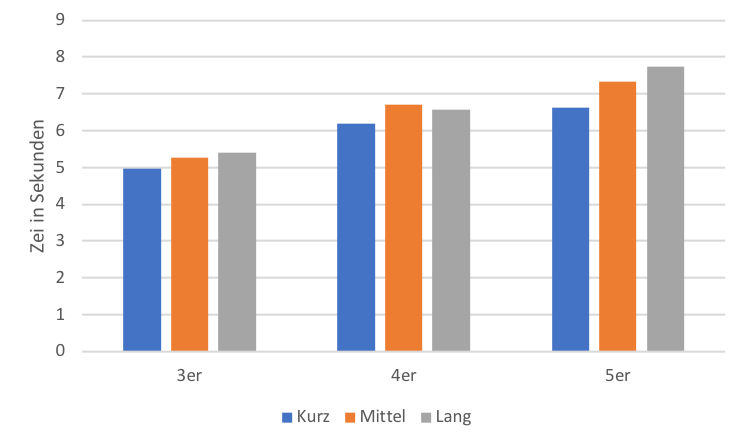
\includegraphics[width=0.8\textwidth]{pics/analyse/algo/ZeitbenoetigtSignalMuster.png}
	\caption{Durchschnittlich ben{\"o}tigte Zeit der Probanden, um ein Signal eines Musters zu erkennen}
	\label{fig:ZeitbenoetigtSignalMuster}
\end{figure}
Im Gegensatz zu der ben{\"o}tigten Zeit beim Algorithmus \autoref{fig:ZeitDurchschnitt}, hat man f{\"u}r jeden Muster-Typen der ein weiteres Signal hinzugef{\"u}gt hat, mehr Zeit ben{\"o}tigt um ein Signal zu erkennen \autoref{fig:ZeitbenoetigtSignalMuster}. 
Die Zeiten f{\"u}r die Muster mit drei Signalen haben sogar eine bessere Zeit als die letzte Iteration vom Algorithmus. 
Alle Signaltypen bei dem dreier Muster haben eine {\"a}hnliche Durchschnittliche Erkennungszeit von f{\"u}nf Sekunden.
%Im Vergleich der Signaltypen bei den dreier Muster-Typen untereinander, wurden unter den dreier Signaltypen jeweils eine Durschnittliche Zeit von ca f{\"u}nf Sekunden ben{\"o}tigt.
Man kann gut erkennen, wie bei den vierer und f{\"u}nfer Muster jeweils die Signaltypen um eine Sekunde mehr Zeit ben{\"o}tigen um diese zu erkennnen, als die dreier Muster.

\begin{table}[]
\centering
\caption{Erkennungsrate (und Standardabweichung) der Mustertypen. Dabei wurden die Genetischen und Generischen Signale miteinander vergliechen}
\label{anova}
\begin{tabular}{l|ll}
              & Genetisch     & Generisch     \\ \hline
3 Vibrationen & 0,817 (0,135) & 0,786 (0,106) \\
4 Vibrationen & 0,771 (0,148) & 0,729 (0,147) \\
5 Vibrationen & 0,756 (0,123) & 0,686 (0,138)
\end{tabular}
\end{table}

Mittels einer Varianzanalyse habe man die Werte aus der \autoref{anova} bestimmt. 
Es hat sich ergeben, dass die Probanden signifikant schlechter abgeschnitten sind, als man sie mit einem komplexeren Mustern konfrontiert hat, im Vergleich zu weniger komplexeren Mustern. 
Eine weitere Erkentniss ist gewesen, dass die genetischen Muster besser erkannt wurden als die generischen Muster.














